\begin{center}
\begin{LARGE}
\title{\textbf{Maciej Jamroży}}
\end{LARGE}
\end{center}
\section{Uprawa monstery}

\subsection{Wymagania}
\begin{justify}
\textbf{Monstera} - każdy z nas ma ten kwiat w swoim domu. Swoją popularność zawdzięcza najprawdopodobniej niskim wymaganiom, a co za tym idzie łatwością w uprawie.

Optymalna temparatura do jej uprawy to 20 stopni C. ale bez większych problemów przystosuje się do temperatury z zakresy 15-30 stopni C. Znosi nawet suche powietrze, wystraczy podlewać ją raz w tygodniu, a przesadzać raz do roku w okresie wiosennym.

Roślina ta bedzię rozwijała się znacznie lepiej jeśli zapewnimy jej podporę.
\end{justify}

\subsection{Ciekawostka}
Monstera rosnąca w idelanych warunkach może wydać owoc, w postaci miąższowatej jagody, o eliptycznym kształcie. Owoc (przykładowo monstery dziurawej) zawiera dużą ilość dopaminy!

\subsection{Istnieją też inne odmiany monster:}
    \begin{itemize}
        \item[-] monstera \emph{deliciosa}
        \item[-]monstera \emph{adansonii}
        \item[-]monstera \emph{tetrasperma}
        \item[-]monstera \emph{dubia}
        \item[-]monstera \emph{dissecta}
    \end{itemize}
\subsection{Jeśli chcesz poprawnie przesadzić swoją monsterę to powinieneś podążać za tymi wskazówkami:}
    \begin{enumerate}
        \item Wybierz nową doniczkę, o kilka centymetrów większą od dotychczasowej.
        \item Monsterę zawsze sadzimy do doniczki z otworem oraz odpowiednią ilością drenażu.
        \item Nie zapomnij o podporze!
        \item Najlepiej użyć dobrze przepuszczalnej ziemi do kwiatków doniczkowych.
    \end{enumerate}

\subsection{Najpiękniejsze odmiany monstery to monstera \emph{Variegata} oraz monstera \emph{Thai Constellation}}
\begin{figure}[hbt!]
    \begin{minipage}{0.5\textwidth}
        \centering
        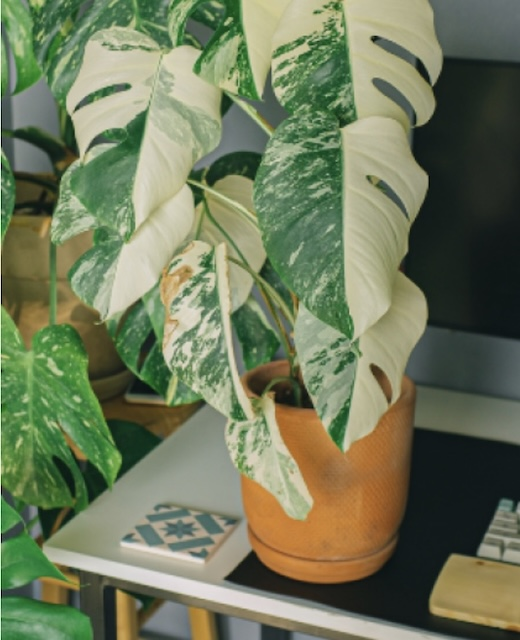
\includegraphics[width=\linewidth]{pictures/monsteravariegata.jpeg}
        \caption{Monstera \emph{Variegata}}
    \end{minipage}%
    \begin{minipage}{0.5\textwidth}
        \centering
        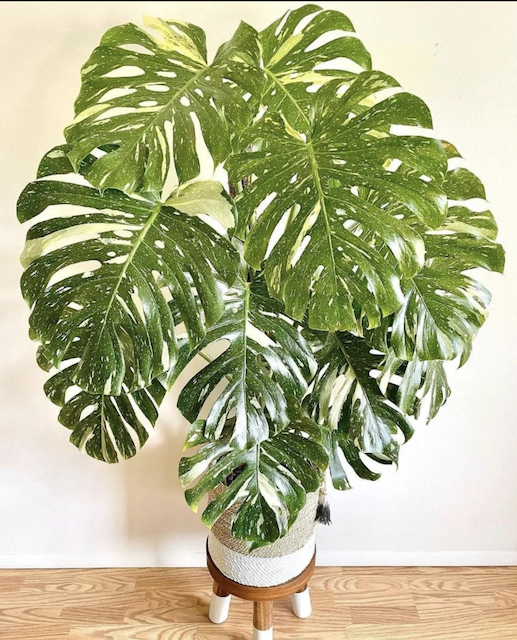
\includegraphics[width=\linewidth]{pictures/monsterathaiconst.png}
        \caption{Monstera \emph{Thai Constellation}}
    \end{minipage}
\end{figure}

\subsection{Czy owoc monstery jest pożywny?}

\begin{table}[ht]
\centering
\begin{tabular}{|l|l|}
\hline
Wartość energetyczna & 308 kJ (73,7 kcal) \\ \hline
Białka               & 1,8 g              \\ \hline
Węglowodany          & 16,2 g             \\ \hline
Tłuszcze             & 0,2 g              \\ \hline
Woda                 & 77,9 g             \\ \hline
\end{tabular}
\caption{Wartości odżywcze owoców monstery dziurawej w 100g}
\label{tab:my-table}
\end{table}

\subsection{Na wypadek, gdyby ktoś zapomniał:}
Rozwiązanie równania kwadratowego $ax^2 + bx + c = 0$ wyraża się wzorem:
\[ x = \frac{{-b \pm \sqrt{{b^2-4ac}}}}{{2a}} \]